\section{Features}
We are now going to highlight some of the most important features of {\germinate}. All features shown in this section are applicable across various data types and pages.

\subsection{User interface language}
\label{sec:features:language-selector}
{\germinate} fully supports internationalization. This means that the interface can be translated into any number of languages. By default, {\germinate} is distributed in English. Depending on the configuration of {\germinate}, other languages may be available. You can switch between them by selecting a language from the first dropdown box shown in Figure \ref{fig:overview:home}C.

\subsection{Menu}
\label{sec:features:menu}
{\germinate}'s main menu (see Figure \ref{fig:overview:home}A) is positioned along the left of the web interface on desktops, although it may collapse into an expandable menu along the top on smaller devices. Clicking on a submenu will expand the corresponding category whereas selecting a menu item will navigate to that page.

Please note, that depending on the configuration of the {\germinate} instance you are using, the menu might have a different structure.

\subsection{Data filtering}
\label{sec:features:filtering}
A lot of tables you encounter in {\germinate} support filtering based on columns. These tables will have a filter icon in the top-left corner which, when clicked on, opens the table column filters.

The filter interface can be seen in Figure \ref{fig:features:filtering}. Each row represents a restriction. It consists of a table column, a comparison operator and, depending on this operator, either one or two values. Multiple rows are combined with boolean combinations. By default the individual filters are combined with a boolean "And", meaning that all of them have to be true at the same time. You can switch this to a boolean "Or" to get results where at least one of the individual filters is fulfilled. Once this filter is applied, the table will only show items that match the given overall filter query.

\begin{figure}
	\centering
	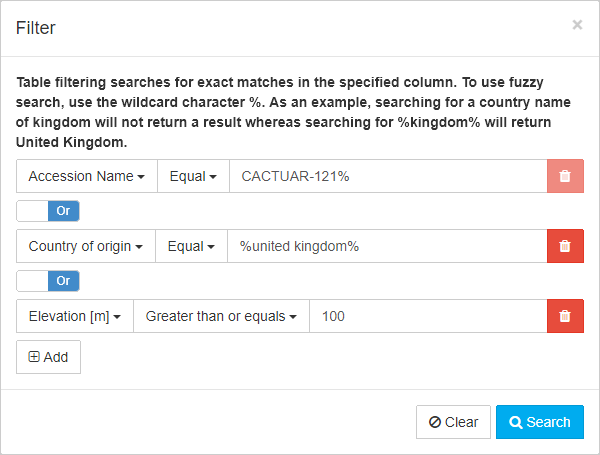
\includegraphics[width=0.5\linewidth]{img/features/table-filtering.png}
	\caption{The table filter interface allows you to define boolean combinations of restrictions for the columns. These support wildcards as well as a variety of different comparison types.}
	\label{fig:features:filtering}
\end{figure}

This is a particularly useful feature if you want to find items that, e.g., are from a specific country, or that have a phenotype value within a certain range. The resulting items can then be marked or put into a group.

\subsection{Search}
\label{sec:features:search}
{\germinate} supports full-text search across various data types and columns within this type. You can search by typing a search query into the text box shown in Figure \ref{fig:overview:home}B. Upon search, {\germinate} shows the search results page. This page shows all matching database objects grouped into categories, each category representing a different data type. Figure \ref{fig:features:search} shows an example of the search results that {\germinate} provides. The number of matching items is shown for each section on the right. Upon expanding of a section, a result table will show the matching database items. You can then either download the data, mark specific items (\cf Section \ref{sec:features:marked-items}) or filter down further by adjusting the search criteria in the table filter (\cf Section \ref{sec:features:filtering}).

\begin{figure}
	\centering
	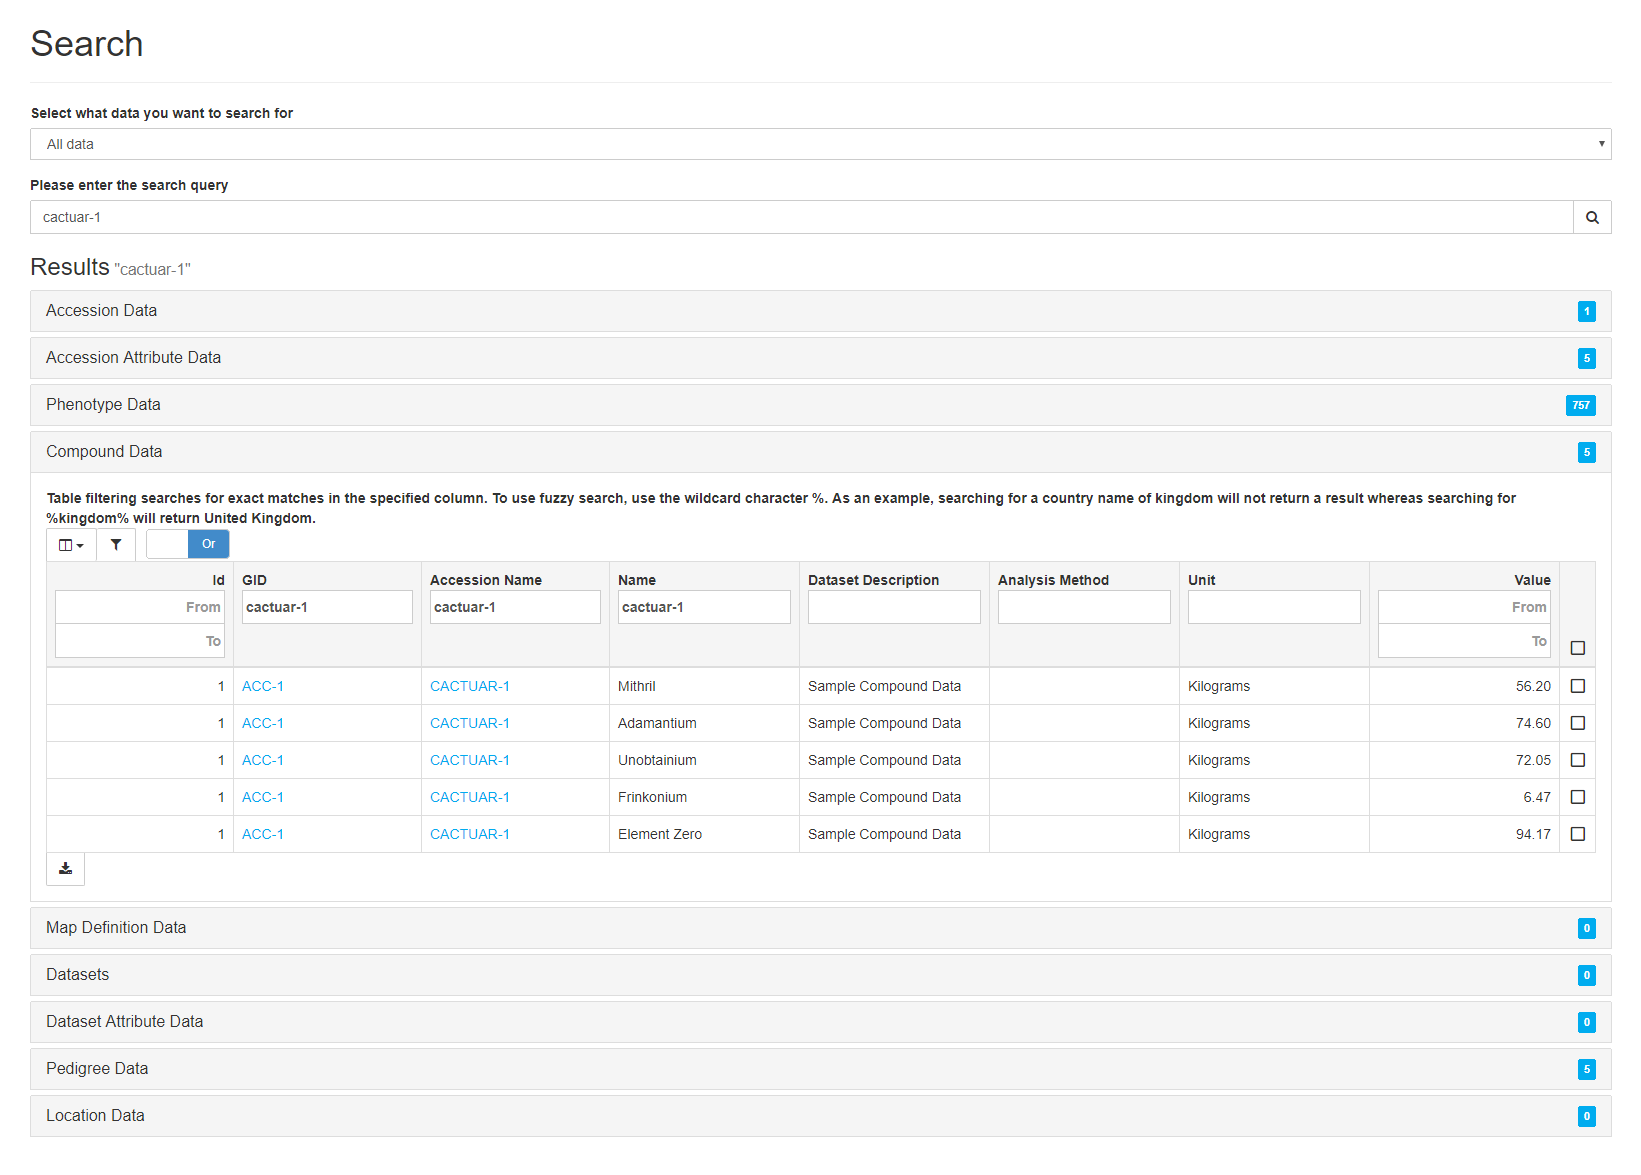
\includegraphics[width=0.85\linewidth]{img/features/search.png}
	\caption{The search results page for the search term "cactuar-1". Results are grouped into categories with the number of matching database items highlighted. The result tables itself can be filtered further to restrict the number of results. In this example the "Compound Data" section is expanded and shows the five results that match the search query.}
	\label{fig:features:search}
\end{figure}

\subsection{Groups}
In {\germinate} we define the concept of a group to be an arbitrary grouping of database items of a certain type. {\germinate} supports groups of \textit{accessions}, \textit{markers} and \textit{locations}. These groups can be pre-created by an administrator or user-defined, which means that you can create your own groups (assuming user authentication is enabled).

The purpose of these groups becomes clear once you start exporting data. All types of data can either be exported for the whole dataset or the data can be subset into smaller chunks by selecting a single or a selection of groups. The exported data will then contain information about the selected groups only.

An example of this is shown in Figure \ref{fig:features:group-subselection} where we selected a group of accessions (192 out of 2000 accessions) and a group containing a single marker (out of 5000). The resulting data file will consequently contain at most 192 rows and at most a single column of data (it may contain less, if the selected database items are not actually part of the selected dataset).

\begin{figure}
	\centering
	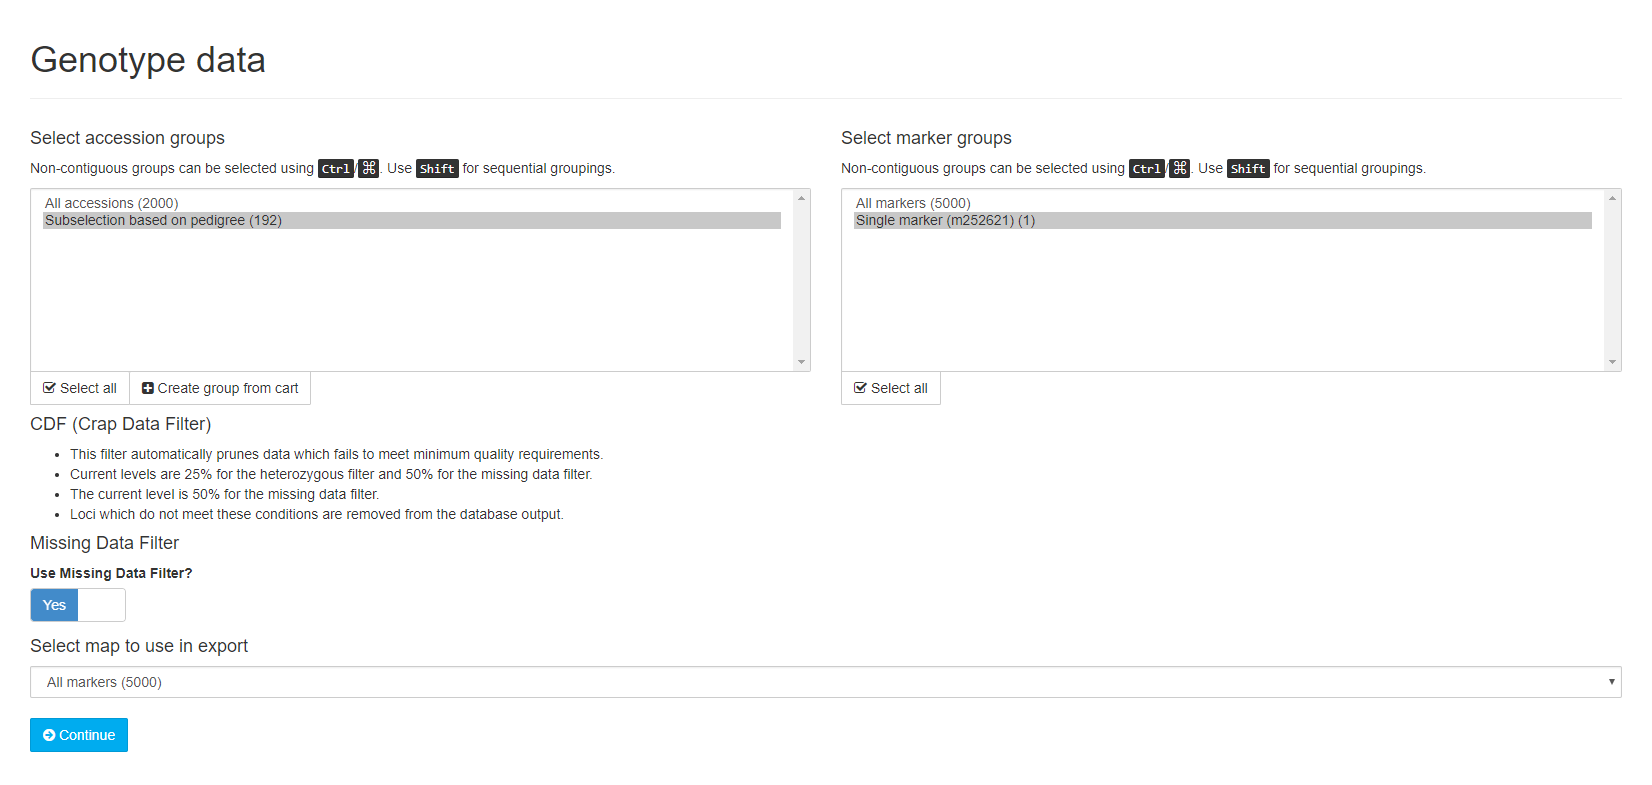
\includegraphics[width=0.85\linewidth]{img/features/group-subselection.png}
	\caption{Example of the group sub-selection feature: You can select both accession and marker groups during the genotypic data export process to subset the dataset.}
	\label{fig:features:group-subselection}
\end{figure}

\subsubsection{Creating a group}
\textit{This section is only applicable if the {\germinate} instance you are using has user authentication enabled.}\\
\\
In addition to using the predefined groups, you can create new groups of your own. There are multiple ways in which you can create a new group and add items to it. One option is to go to the \textit{Groups} page of {\germinate}. This page shows you all the existing groups in a table and upon selection, shows you its group members. Figure \ref{fig:features:groups-page} shows you an example of what the groups page can look like. In this example, {\germinate} contains 118 different groups that the current user can see. New groups can be added and existing ones deleted by pressing the buttons below the groups table (Figure \ref{fig:features:groups-page}A). Deleting a group requires you to select the checkbox in the corresponding table row as well as to have sufficient permissions to do so. When creating a new group you will be asked to select the group type and to decide on a name for the group. When you do so, the group will be associated with your user account.

Once this is done, the group will be created and {\germinate} will automatically select it and show the group members table (empty at this point) below the groups table. You can now manipulate the group itself by adding and removing members using the buttons below the table as shown in Figure \ref{fig:features:groups-page}C.

\begin{figure}
	\centering
	\begin{subfigure}[b]{0.3\linewidth}
		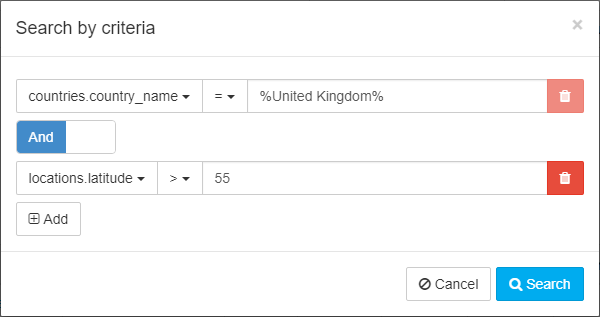
\includegraphics[width=1\linewidth]{img/features/groups-search-query.png}
		\caption{Query}
		\label{fig:features:groups-search-query}
	\end{subfigure}
	\begin{subfigure}[b]{0.68\linewidth}
		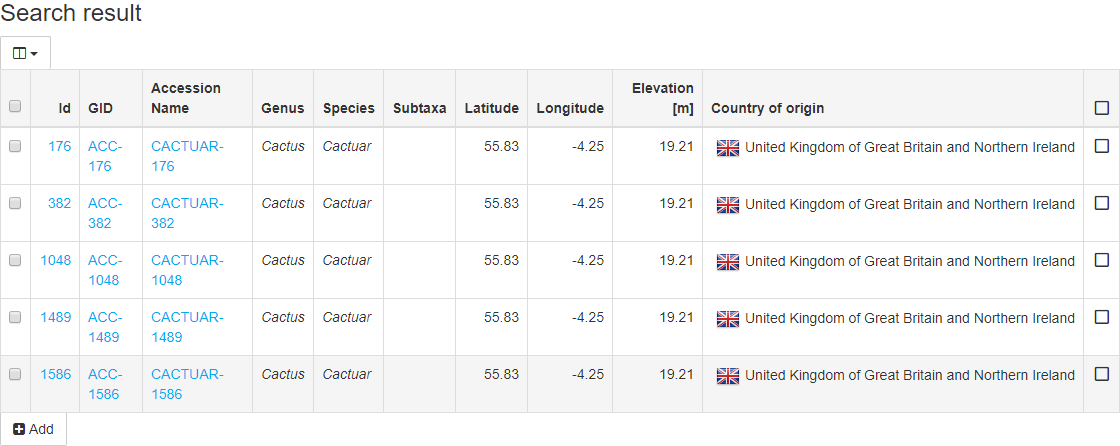
\includegraphics[width=1\linewidth]{img/features/groups-search-result.png}
		\caption{Result}
		\label{fig:features:groups-search-result}
	\end{subfigure}
	\caption{The group member search interface. (A) shows the boolean query interface where you can define the attributes an item needs to fulfil. In this case, the accession has to be collected in the UK at a latitude larger than 55. (B) The table showing the matching items. There are five accessions that match the query.}
	\label{fig:features:groups-search}
\end{figure}

Adding members to an existing group can be achieved in two ways. You can upload a list of those items from a text file or your clipboard and {\germinate} will look these items up based on their identifier. Once found they will be added to the group. The other option is to use a boolean search feature that is similar to the way the table filtering works (\cf Section \ref{sec:features:filtering}). You can choose fields from the database tables and specify values that the items in questions should equal, smaller or larger to. Figure \ref{fig:features:groups-search} shows what the group member search interface looks like. The query is specified in Figure \ref{fig:features:groups-search-query} and the result shown in Figure \ref{fig:features:groups-search-result}.

Groups can be made public so that other users have the option to use them as well. If you decide to make your group public, toggle the switch button shown in Figure \ref{fig:features:groups-page}B.

\begin{figure}
	\centering
	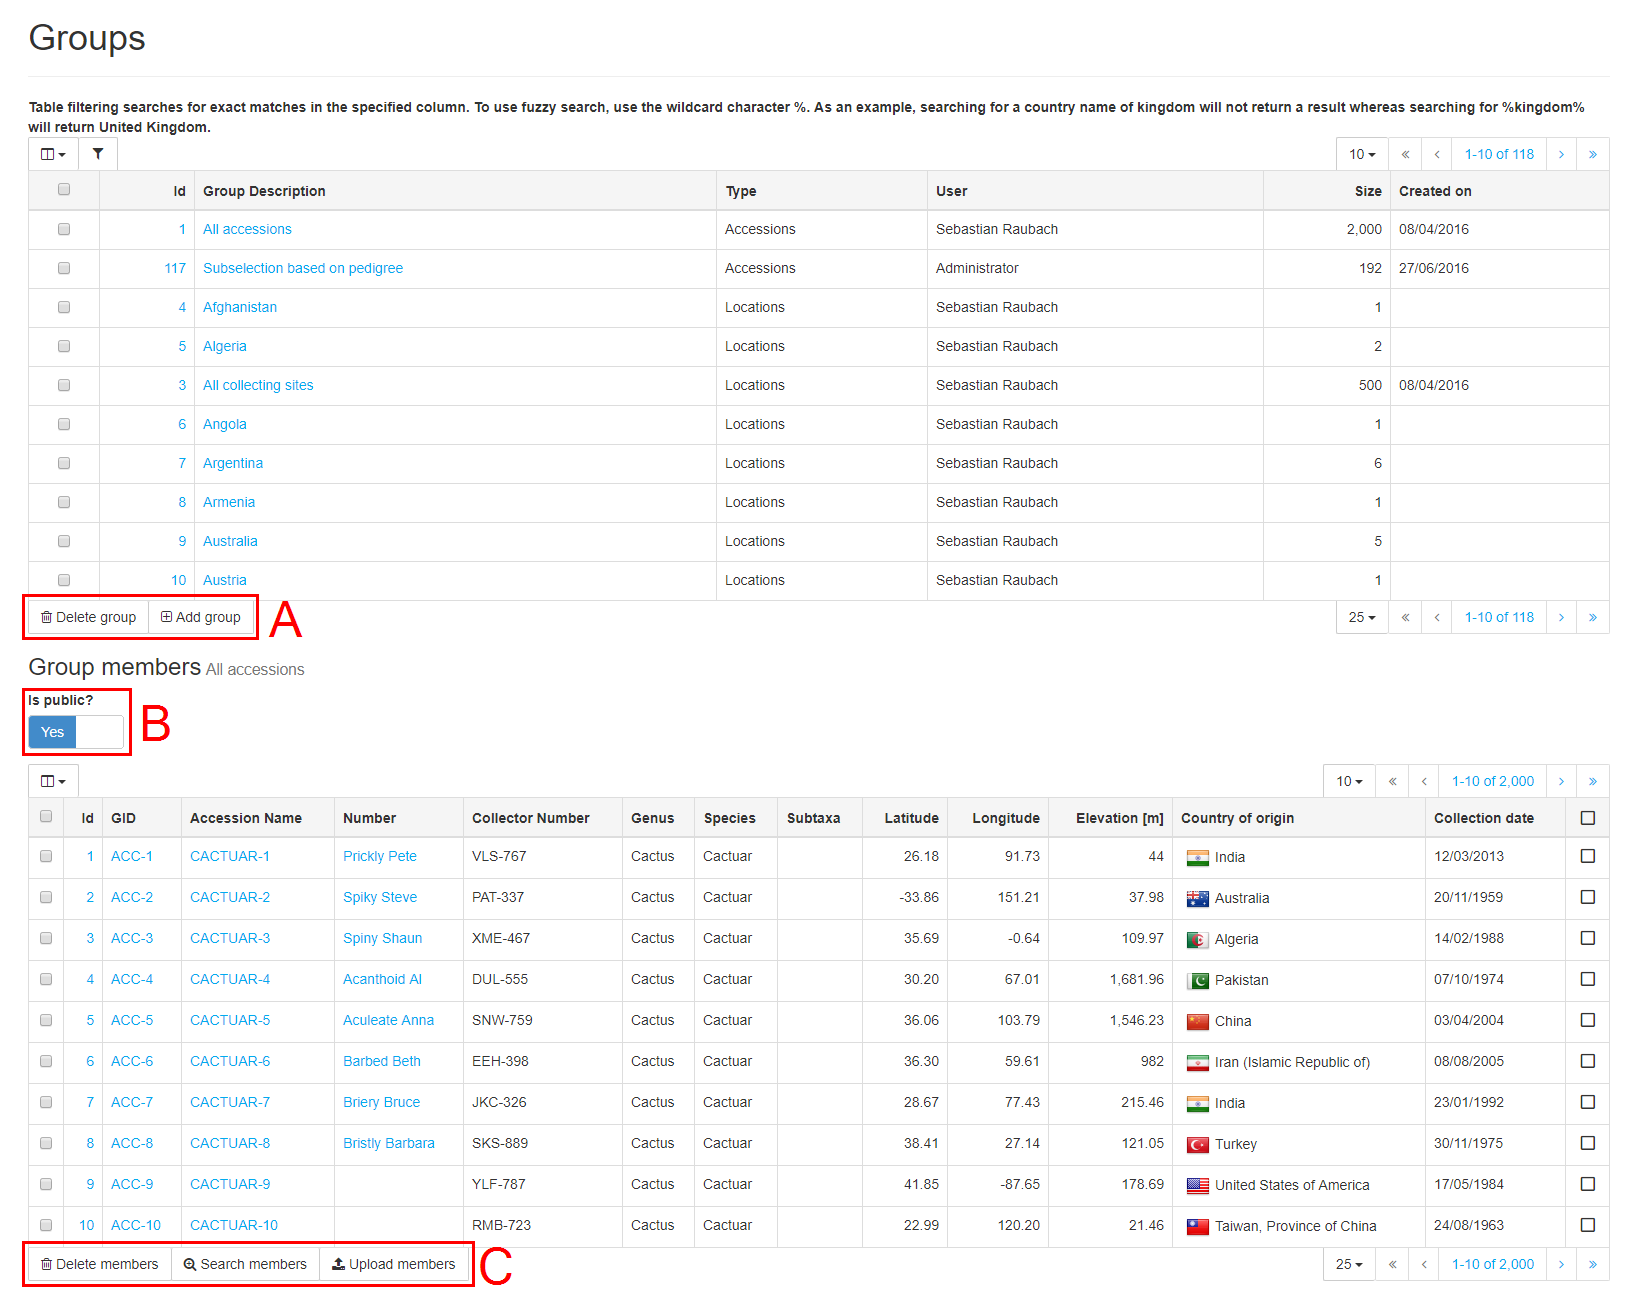
\includegraphics[width=0.85\linewidth]{img/features/groups-page.png}
	\caption{The groups page has many ways in which you can manipulate existing groups and create new groups. The top table shows all the groups that are visible to the current user. The bottom table shows the members of this group, \ie the database items that are part of it; depending on the type of the group, this can be either \textit{accessions}, \textit{markers} or \textit{locations}. (A) Groups can be added and deleted by clicking on the buttons located just below the groups table. Deleting groups requires the checkbox of the corresponding table row to be selected. (B) The group visibility can be changed by toggling this switch. A public group is visible to every user whereas an invisible group is only visible to the owner. (C) Group members can be added and removed by clicking on the buttons below the group member table.}
	\label{fig:features:groups-page}
\end{figure}

\subsubsection{Marked item lists}
\label{sec:features:marked-items}

Another useful feature of {\germinate} is the concept of \textit{marked item lists}. A marked item is either an accession, a marker or a location that is of interest to the user. While you are browsing the page, a lot of the tables will have a checkbox column as the last column which you can use to mark certain items. {\germinate} will keep track of these items for you.

To see how many items you currently have marked, you can click on the menu item as shown in Figure \ref{fig:features:marked-items-dropdown} or go directly to the marked item lists page that is shown in Figure \ref{fig:features:marked-items-page}.

Once you have marked all the items that you are interested in, you can create a group of these items and use them to export data against them. To create a group, you can either go to the marked item lists page or by clicking on the header of the checkbox column and selecting "Create group from selection" (see Figure \ref{fig:features:marked-items-context}).

\begin{figure}
	\centering
	\begin{subfigure}[b]{0.2\linewidth}
		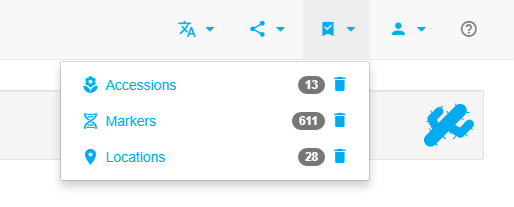
\includegraphics[width=1\linewidth]{img/features/item-list-dropdown.png}
		\caption{Dropdown}
		\label{fig:features:marked-items-dropdown}
	\end{subfigure}
	\begin{subfigure}[b]{0.58\linewidth}
		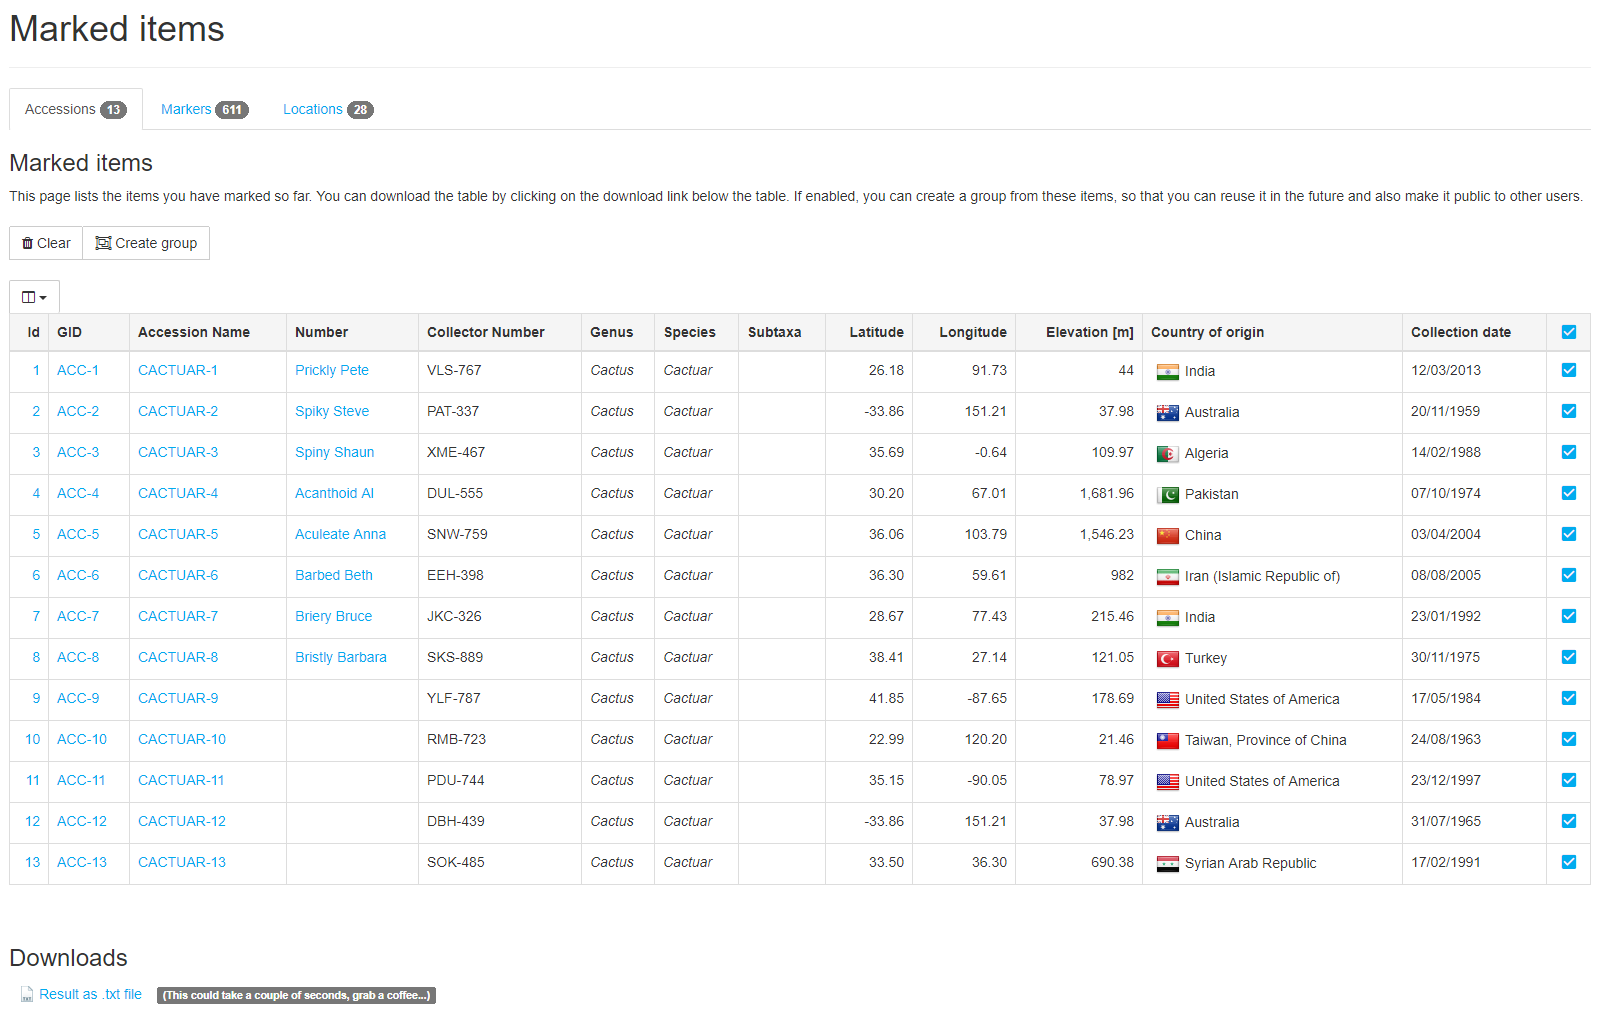
\includegraphics[width=1\linewidth]{img/features/item-list-page.png}
		\caption{Page}
		\label{fig:features:marked-items-page}
	\end{subfigure}
	\begin{subfigure}[b]{0.2\linewidth}
		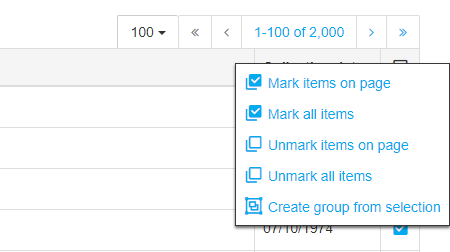
\includegraphics[width=1\linewidth]{img/features/item-list-context-create-group.png}
		\caption{Context menu}
		\label{fig:features:marked-items-context}
	\end{subfigure}
	\caption{The marked item lists keep track of items of interest. (A) The dropdown menu shows a quick overview of how many items of each type are currently marked. The bin icon lets you easily empty the marked item list of a certain type. (B) The actual marked item lists page shows three tabs, one for each item type. The table under each tab shows all marked items of this type. You can either download this information or create a group from the list (if this is enabled). (C) Many tables have a checkbox column that you can use to mark/unmark items. You can also create a group from this context menu (if this is enabled).}
\end{figure}

\subsection{Charts}
Most of the charts we use in {\germinate} are custom-built for this interface and therefore closely integrate with the way {\germinate} operates. All charts will offer some kind of interactivity. This can range from simple tooltips to the ability to select data points with a lasso. All charts can be downloaded as a Portable Network Graphics (PNG) or a Scalable Vector Graphics (SVG) file. Additionally, the underlying data for each chart can be downloaded in a tab-delimited data file. If the selection of individual data points is enabled, the selected items can be added to or removed from the marked item list.

\subsection{Help}
\label{sec:features:help}

Whenever you are stuck and are not sure what to do or how to use the web interface, you can click on the last item in Figure \ref{fig:overview:home}C. This will open a popup with information about the page you are looking at. Sometimes this information may provide links to external resources or external tools, other times it will just explain certain parts of the page in more details.

Please note that help information may not be available for all pages. In those cases, the menu item will be disabled. We are trying to make the user interface as intuitive as possible and are working towards adding help information to all the pages. If at any point you have questions about {\germinate} in general or specific features of the web interface, please do not hesitate to contact us on: \href{mailto:germinate@hutton.ac.uk}{germinate@hutton.ac.uk}.